\documentclass[12pt, letterpaper]{article}
\usepackage{graphicx}
\usepackage{amsmath}% For the equation* environment
\title{第二次小组作业}
\PassOptionsToPackage{quiet}{fontspec}
\usepackage[UTF8]{ctex}
\author{Suiran}
\begin{document}
\maketitle

\newpage
\section{第一题}
\subsection{模型}

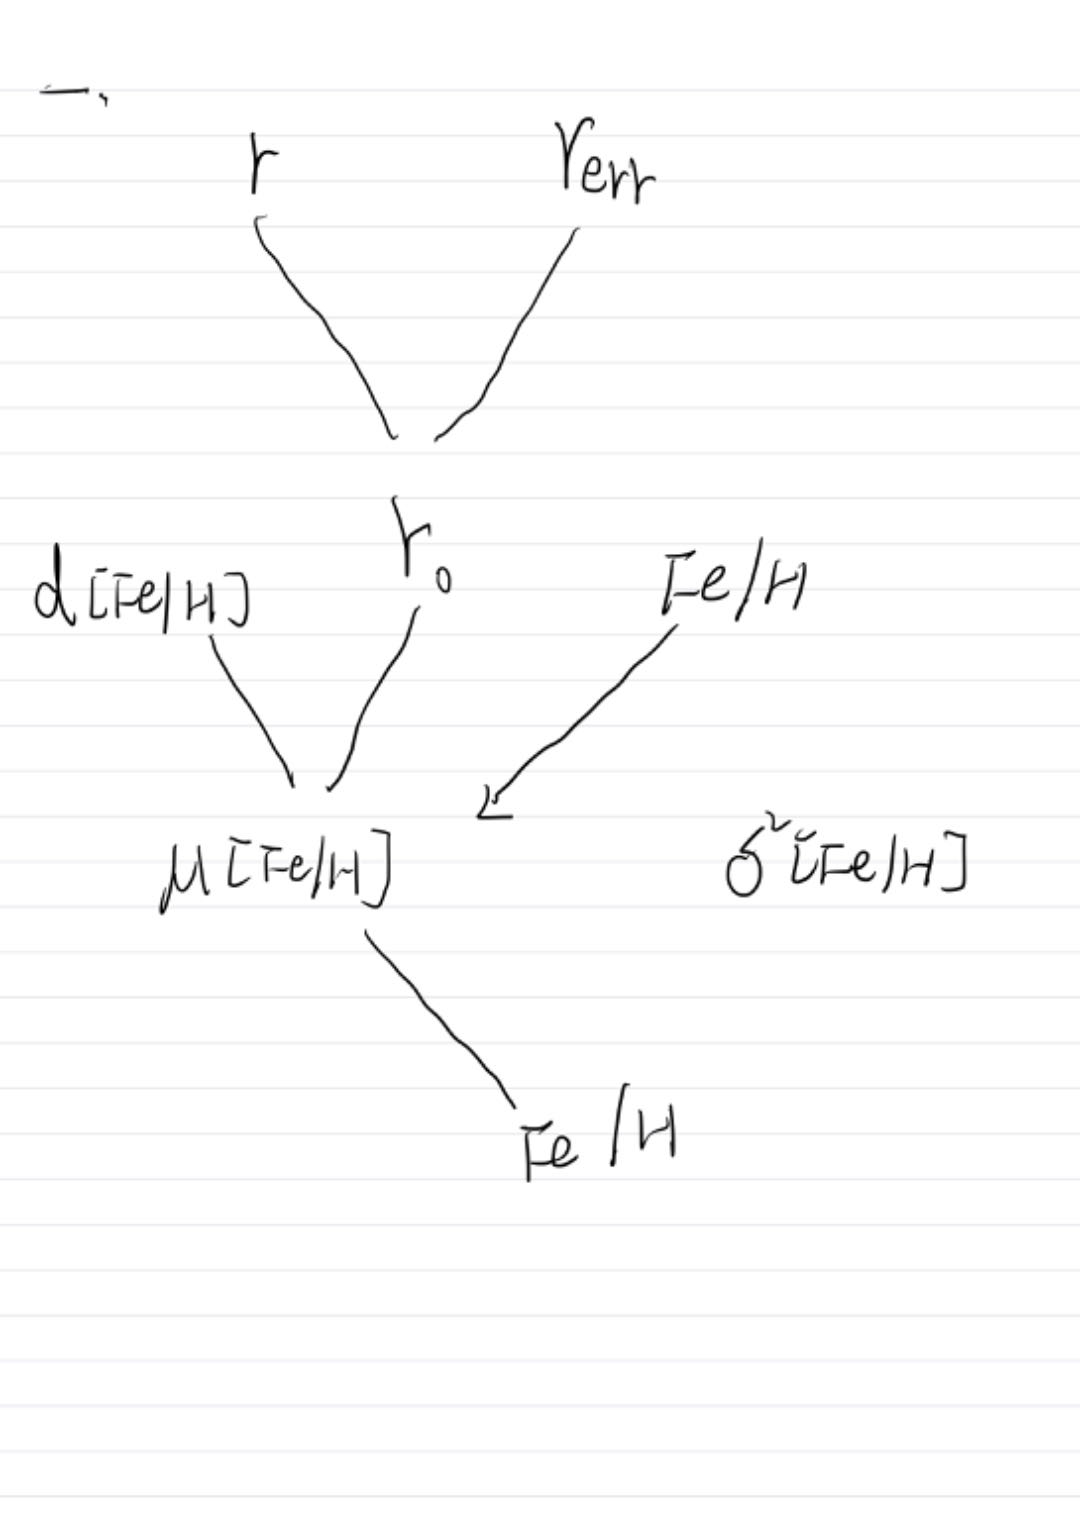
\includegraphics[scale=0.333]{A.png}

后验分布为
\begin{equation}
\begin{split}
	P(d[Fe/H],[Fe/H]_0|[Fe/H], r_0, \sigma^2[Fe/H],r_{err})\\
	\propto \prod_i^nP([Fe/H]_i|\sigma^2[Fe/H], \mu[Fe/H]_i)P(r_0|r, r_{err})\cdot \\
	P(r)P(r_{err})P([Fe/H]_0)P(d[Fe/H]_i)P(\sigma^2[Fe/H]_i)	
\end{split}
\end{equation}
其中满足分布:
\begin{equation}
	P(r_0|r, r_{err})\sim \mathcal{N}(r,r_{err})
\end{equation}
\begin{equation}
	P([Fe/H]_i|\sigma^2[Fe/H], \mu[Fe/H]_i)\sim \mathcal{N}(\sigma^2[Fe/H], \mu[Fe/H]_i)
\end{equation}
\subsection{程序}
另附
\subsection{结果}
结果为$[Fe/H]_0=0.50$,$[d[Fe/H]=-0.07$

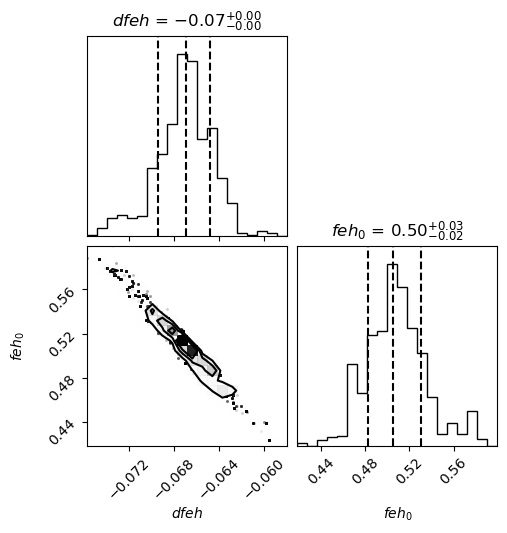
\includegraphics[scale=0.7]{1.png}

%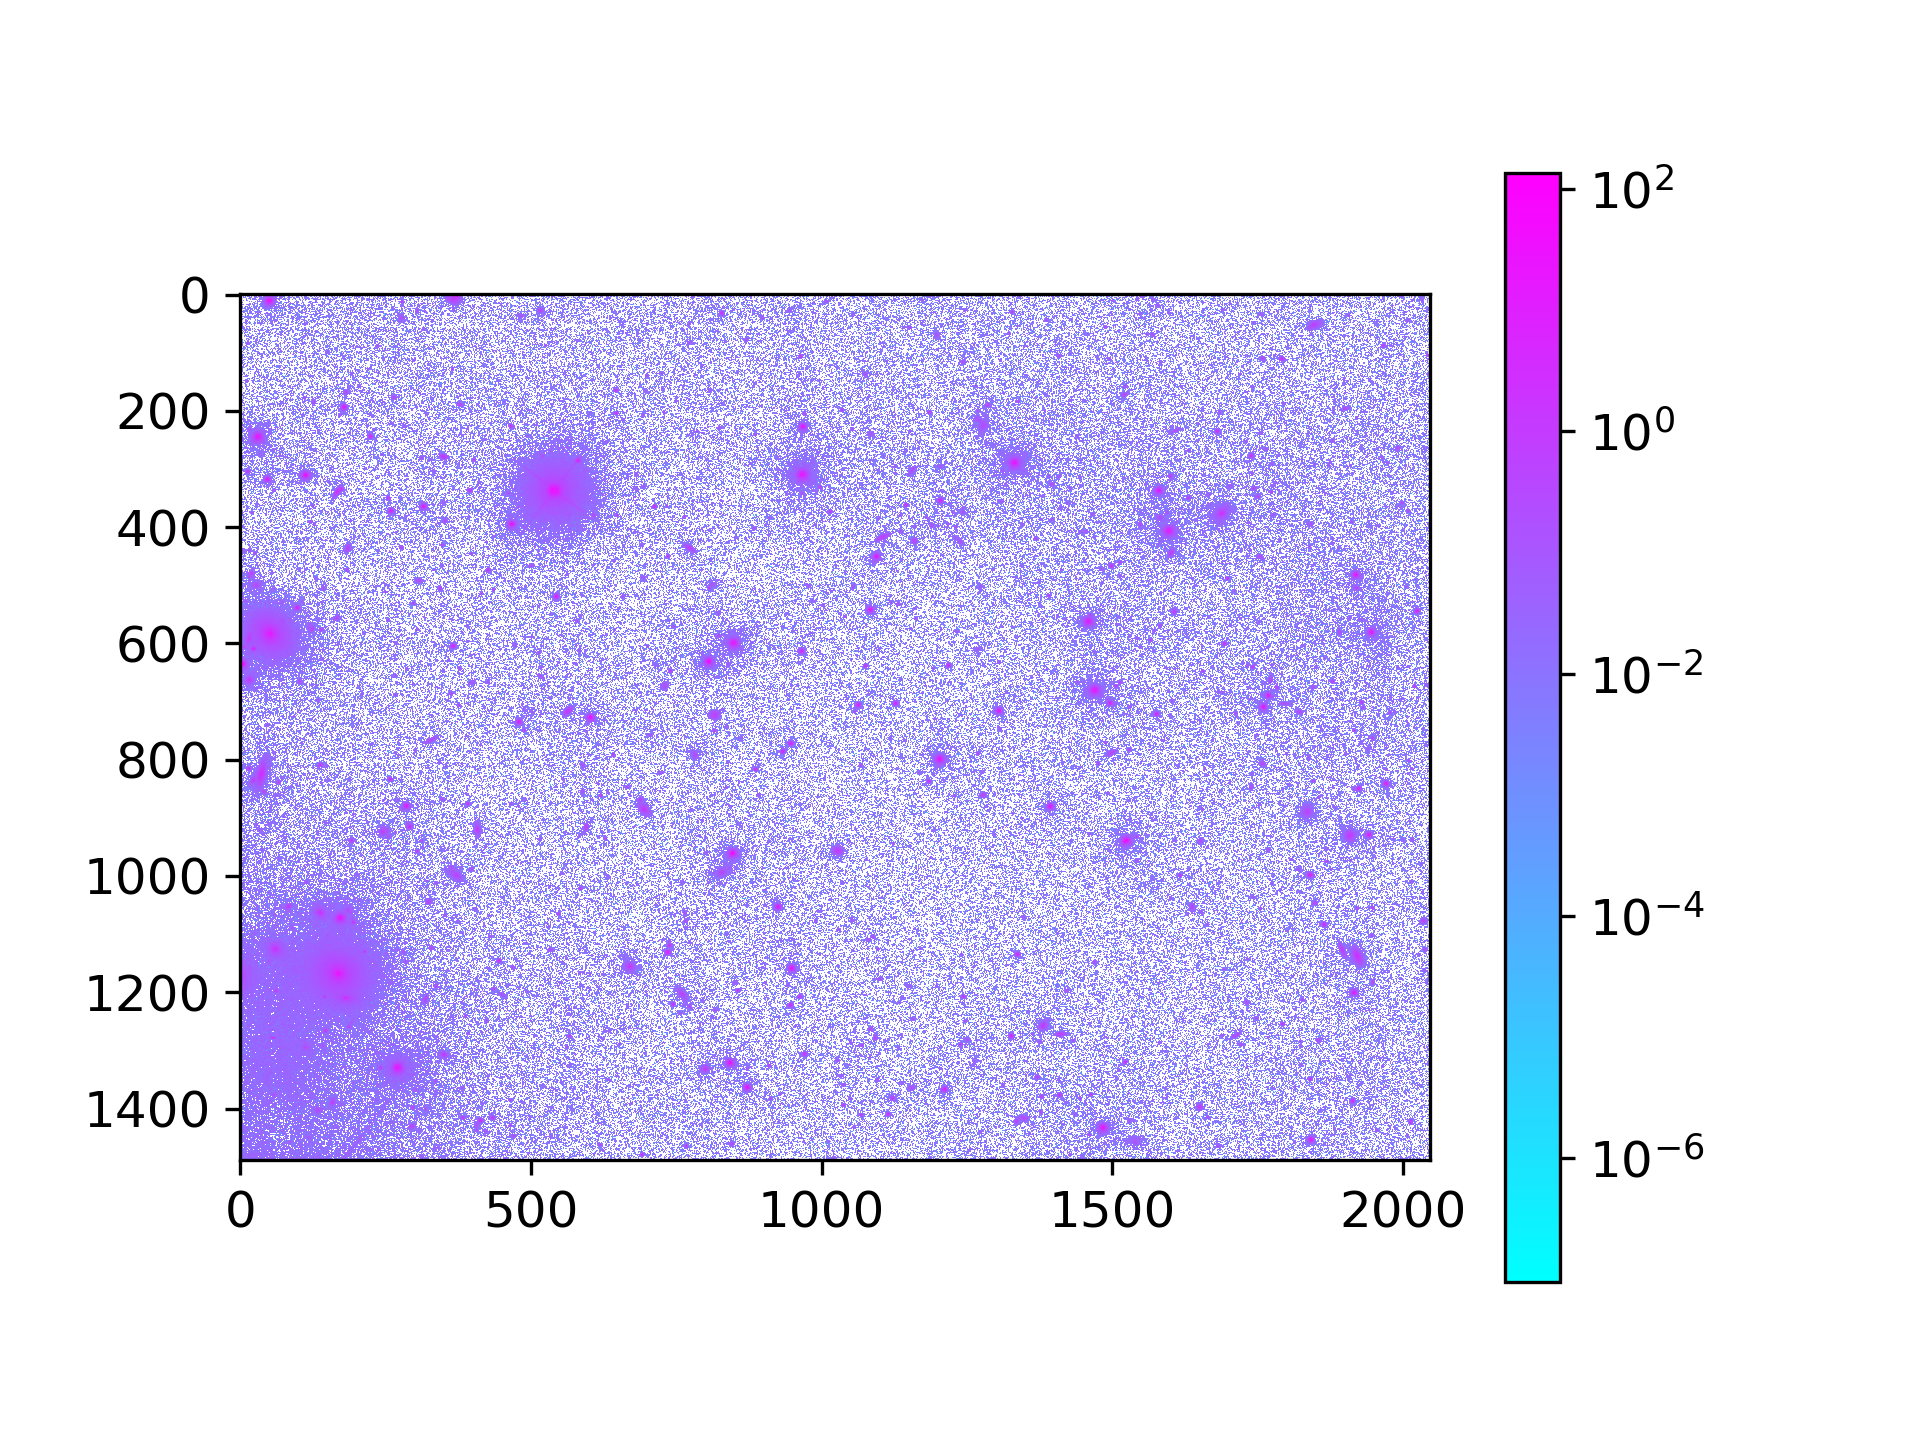
\includegraphics[scale=0.7]{2_1.png}

%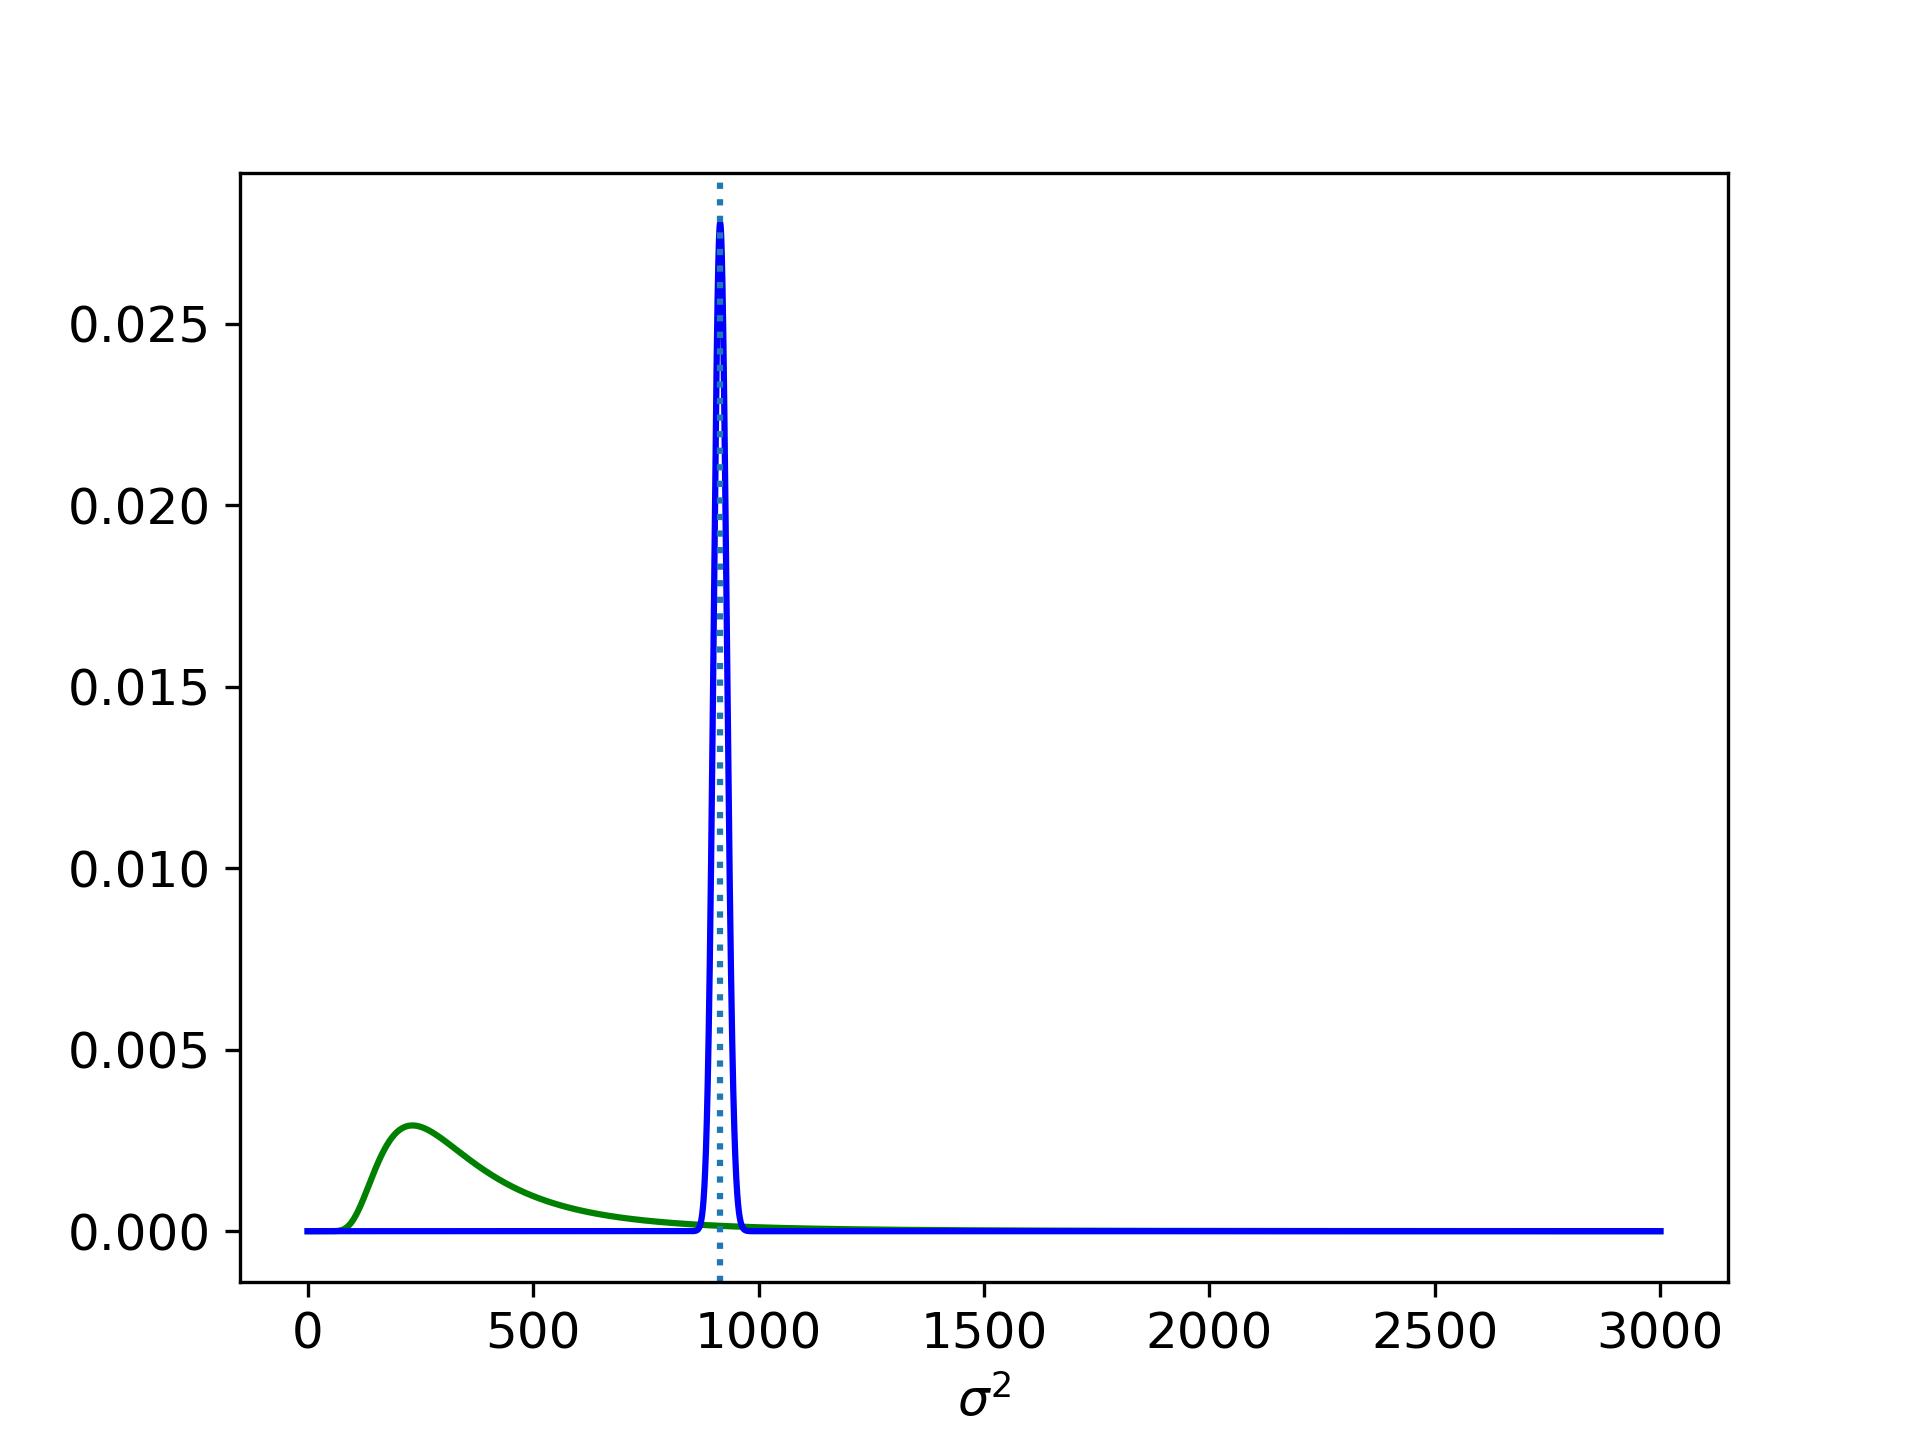
\includegraphics[scale=0.7]{3_3.png}
\section{第二题}
\subsection{模型}

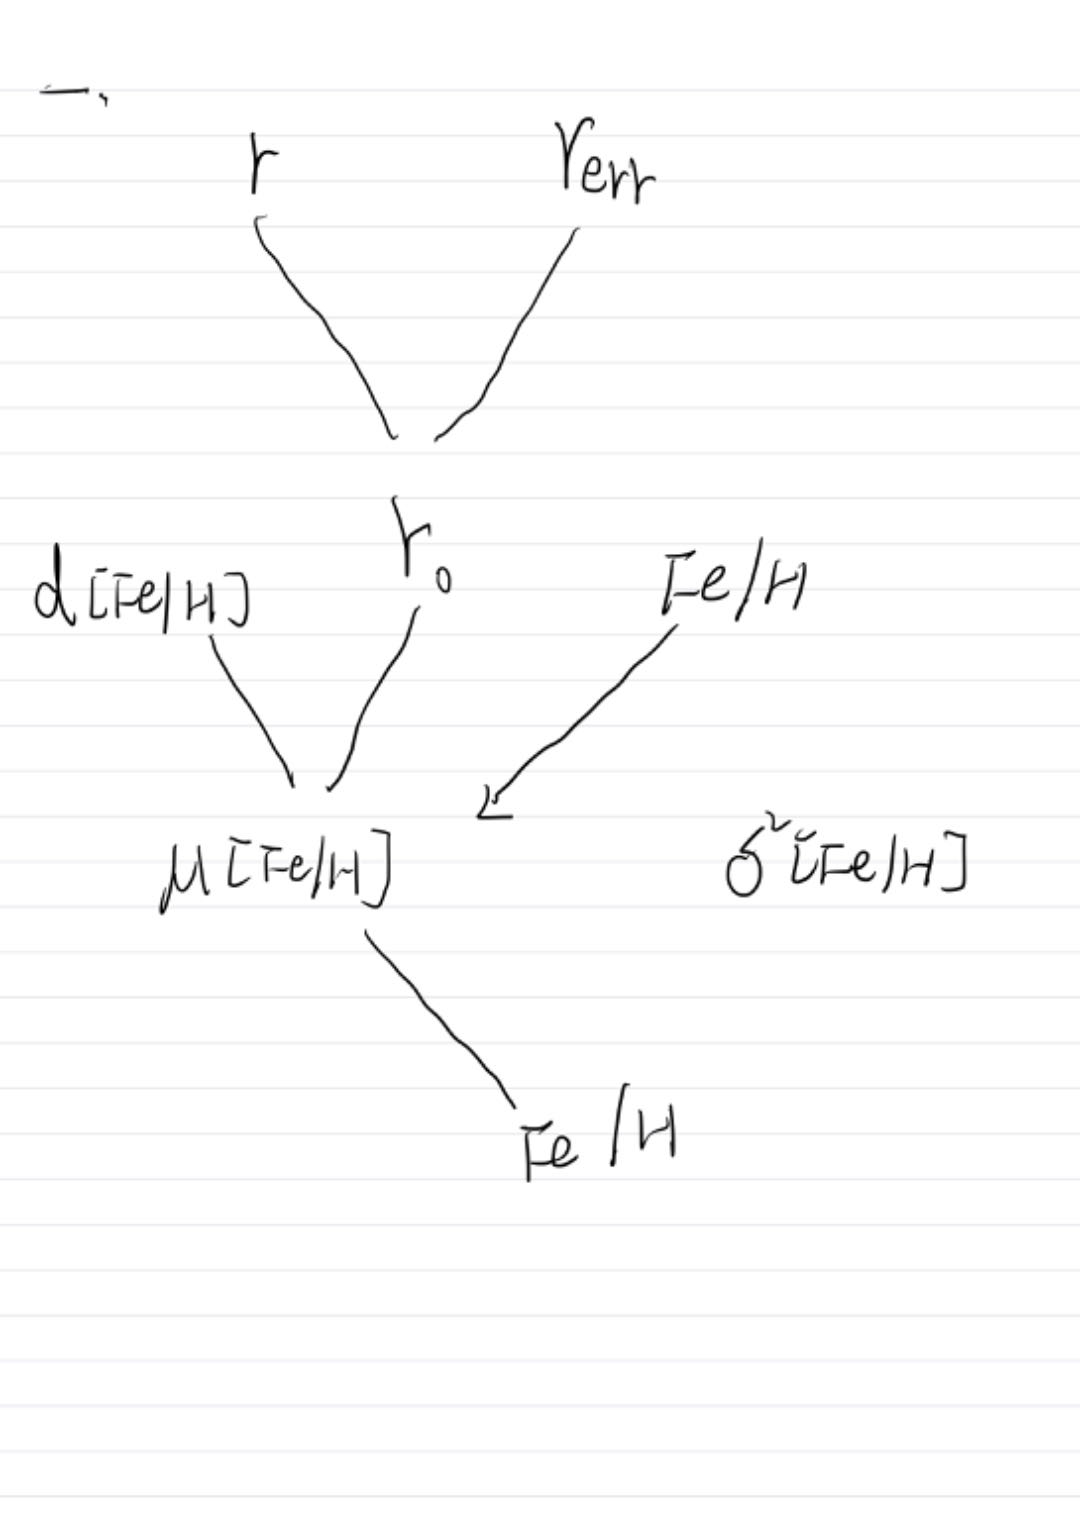
\includegraphics[scale=0.333]{A.png}

后验分布为
\begin{equation}
\begin{split}
	P(hR, a|r, r_{err}, \mu rv)\\
	\propto P(rv|\mu rv, \sigma^2+\epsilon_i^2)P(\sigma^2+\epsilon_i^2|hR, a, r_0)\cdot\\
P(r)P(r_{err})P(\mu rv)
\end{split}
\end{equation}
其中满足分布:
\begin{equation}
	P(r_0|r, r_{err})\sim \mathcal{N}(r,r_{err})
\end{equation}
\begin{equation}
	P(rv|\sigma^2+\epsilon_i^2, \mu rv)\sim \mathcal{N}(\sigma^2+\epsilon, \mu rv)
\end{equation}
\subsection{程序}
另附
\subsection{结果}
结果为$hR=15.01$,$a=2503.40$

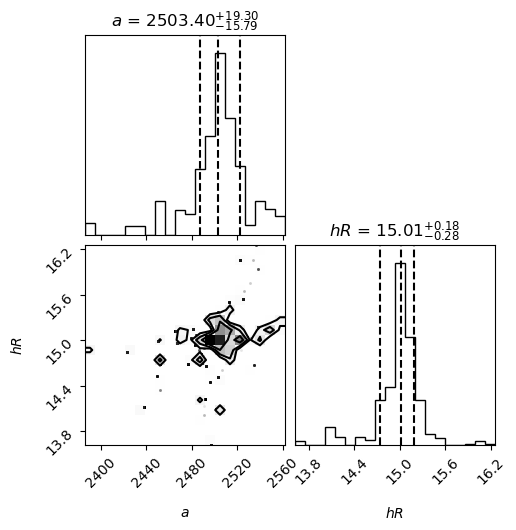
\includegraphics[scale=0.7]{2.png}

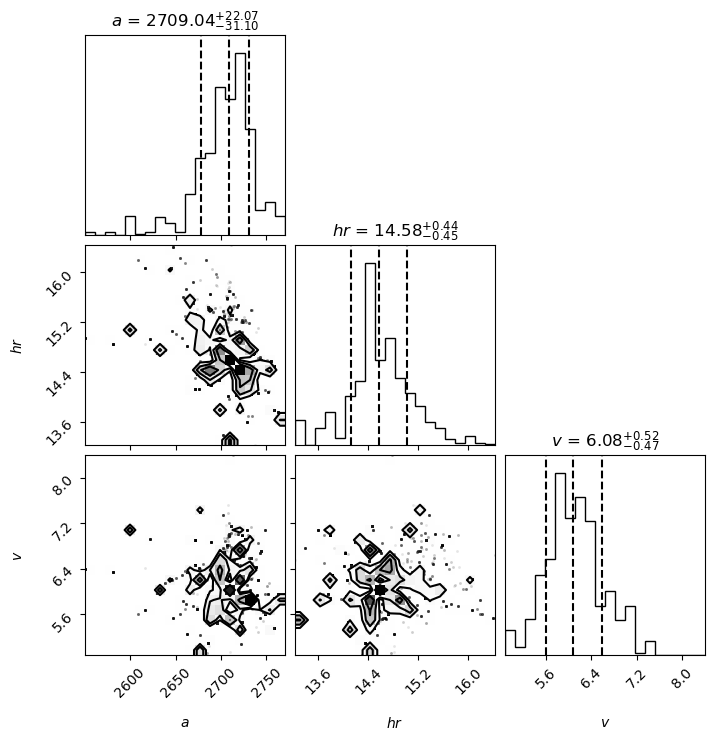
\includegraphics[scale=0.7]{3.png}

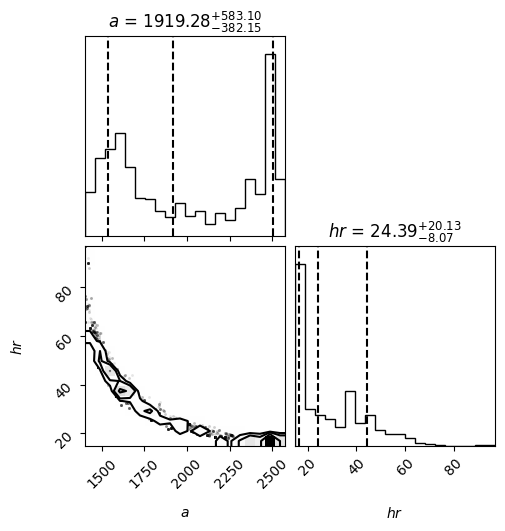
\includegraphics[scale=0.7]{4.jpg}
\end{document}
